\documentclass[11pt]{report}

%packages we want
\usepackage{hyperref}
\hypersetup{
    colorlinks,
    citecolor=black,
    filecolor=black,
    linkcolor=blue,
    urlcolor=blue
}
\usepackage{graphicx}
\DeclareGraphicsExtensions{.pdf,.png,.jpg}
\usepackage{caption}
\usepackage{subcaption}

\usepackage{multicol}
\usepackage{fancyvrb}



%Some helpful commands
\newcommand{\csgt}[0]{\textbf{CS\textgreater\ }}

%Gummi|065|=)
\title{\textbf{\csgt System User Manual}}
\author{Jeb Brooks}
\date{}
\begin{document}

\maketitle

\tableofcontents

\listoffigures

\chapter{Introduction}
The \csgt system is an all in one submission system and grading platform designed primarily for use
with CS coursework. It is designed to support basic grading functionality and auto-grading capabilities.
Additionally it is designed to be extended to support new testing systems through a simple plug-in system
which can hot-load new plugins on a live instance.

This document will attempt to get you familiar with the \csgt system and guide you through using and maintaining
its various features. \csgt provides the following major features:

\begin{itemize}
\item Logical assignment/problem grouping
\item Fully featured grade-book system. Supports adding groups and columns to the grade-book which are not
based on student submitted work (e.g.. Participation Points or Quizzes)
\item Markdown enabled grader comment system.
\item Automatic grading based on unit tests (modifiable via plug-ins)
\item Automatic late grade calculation (modifiable via plug-ins)
\item Built-in wiki support for problem descriptions and notes for graders. The wiki also supports various
permissions levels.
\item Support for command line control of the system.
\item Support for listing currently active tutors and locations so students can get help on problem sets.
\end{itemize}

This document will attempt to guide you through the use of these features. Because not all features are useful to
every class of user this document is divided into three chapters. The \nameref{ch:use} chapter should be
enough for instructors, tutors, and students. The \nameref{ch:admin} chapter will cover topics required to set-up
and maintain the \csgt system. Finally, the \nameref{ch:develop} chapter will cover topics required to develop
new plug-ins and modify the core functionality of the system.


\chapter{Basic Use}
\label{ch:use}
This chapter will attempt to cover all of the basic use cases for the various user situations.
In addition it will describe the built in wiki system which ships with the \csgt system.

\section{General Use}
This section covers general account management.
\subsection{Logging in/Password Recovery}
Most of the features for the site are restricted to registered users. The login button is located in the
top right corner of the page, see Figure \ref{fig:main_page}.

\begin{figure}
\centering

\includegraphics[width=\textwidth,height=\textheight,keepaspectratio]{diagrams/main_page}
\caption{The header of the main page before logging in.}
\label{fig:main_page}
\end{figure}

If you forget your password (and the system has been configured to send emails, see Section \ref{sec:config})
you may recover your password on the login page, shown in Figure \ref{fig:login_page}.

\begin{figure}
\centering
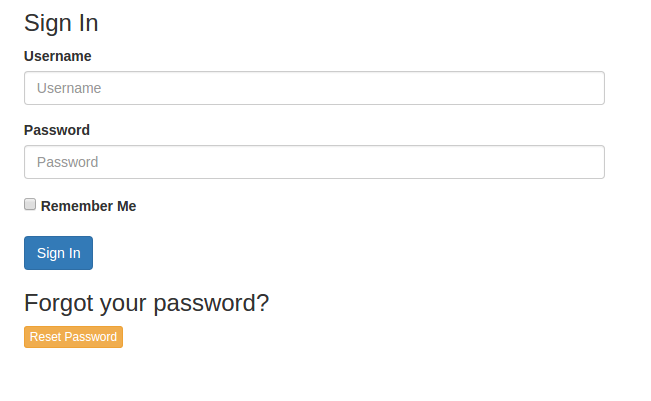
\includegraphics[width=\textwidth,height=\textheight,keepaspectratio]{diagrams/login_page}
\caption{The login page. Reset password is at the bottom.}
\label{fig:login_page}
\end{figure}

\subsection{The Main Navigation Bar}

Most navigation will be done through the use of the main navigation bar at the top of the screen, see
Figure \ref{fig:nav_bar}. The navigation bar's content will change based on the permissions of your
account. Figure \ref{fig:nav_bar} shows an account that occupies all three roles, student, grader, and
instructor.

\begin{figure}[h]
\centering

\includegraphics[width=\textwidth,height=\textheight,keepaspectratio]{diagrams/main_header}
\caption{The main navigation bar}
\label{fig:nav_bar}
\end{figure}

From right to left the links on the navigation bar are:
\begin{description}
\item[Home] Takes you to the main page.
\item[Courses] Presents a drop-down menu which can take you to the homepage for active courses in the system.
\item[Active Grutors] Takes you to a page which shows where the current active grutors are for
courses you are involved with (enrolled, grading, or teaching).
\item[Student] This only appears if you are a student in a course and will present a drop-down that can take
you to the problem submission page for your course or a summary of your grades.
\item[Grader] This only appears for graders and instructors of a course. It presents a drop-down for choosing
which course you want to grade assignments for.
\item[Instructor] This only appears for instructors. It presents a drop-down for which course you want to
edit settings for.
\item[Leave a Comment] Takes you to a feedback page. Feedback provided through this page is sent to the
admin.
\item[Report a Bug] Takes you to the github issues page for the \csgt system.
\item[\textless username\textgreater] Presents a drop-down for account settings and logging out.
\end{description}


\section{Student Use}
The primary actions students will take in \csgt is submitting homework assignments and checking grades.

\subsection{Submitting Homework}
To submit homework start by clicking the \emph{Student} link on the navigation bar and selecting the course
which you want to submit work to. This will bring you to a page like in figure \ref{fig:problem_list}.

\begin{figure}[h]
\centering
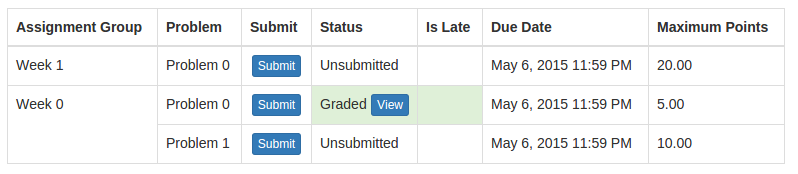
\includegraphics[width=\textwidth,height=\textheight,keepaspectratio]{diagrams/problem_list}
\caption{A list of problems for a course. Problems are grouped by \textbf{Assignment Group}}
\label{fig:problem_list}
\end{figure}

Problems are grouped by \textbf{Assignment Group} which may refer to single weeks or any other logical
grouping of multiple problems. Assignment groups are displayed in reverse order so that the most recently
assigned group is at the top of the list and thus easier to find.

Once you have located the problem you wish to submit click the blue \emph{Submit} button. This will direct
you to a page like in figure \ref{fig:submit_page}.

\begin{figure}
\centering
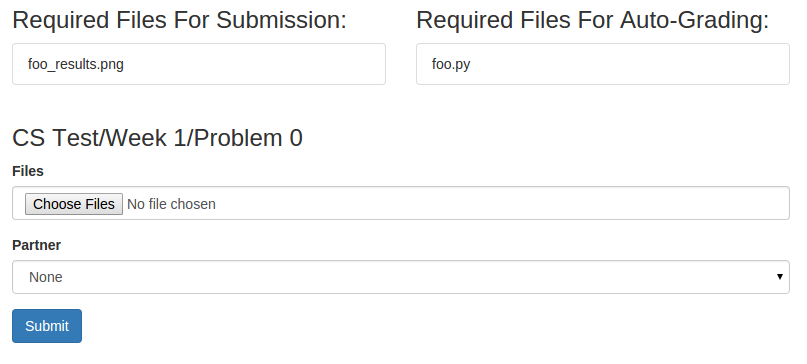
\includegraphics[width=\textwidth,height=\textheight,keepaspectratio]{diagrams/submit_page}
\caption{The page for submitting files for a problem}
\label{fig:submit_page}
\end{figure}

On the submit page there is information about what files are expected, a place for you to choose the
files you are submitting and a drop-down to select an optional partner.

\begin{description}
\item[Required Files For Submission] These files must be present in the set of files you select or else
the system will reject the submission.
\item[Required Files For Auto-Grading] If any of these files are not present the submission will be accepted
but the auto-grader will not run.
\item[Files] Will open a file selection window. To submit multiple files you may either select multiple files in
the window, or submit a zip file. If you need to preserve directory structure submit a zip file.
\item[Partner] A drop-down of all the students in the course for selecting a partner. If you select a partner
your partner does not have to submit the solution as well.
\end{description}

\subsection{Viewing Grades}
There are two ways to view grades. First on the problem list page, see figure \ref{fig:problem_list}, you can
click the \emph{view} button to see the grade and grader comments for an individual problem.

If you want an overview of all of your grades you can go to the \emph{My Grades} page which is under the student
drop-down menu. The My Grades page will display something like in figure \ref{fig:my_grades}.

\begin{figure}
\centering
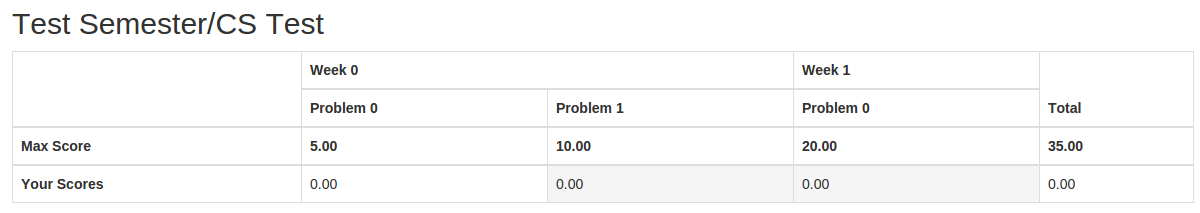
\includegraphics[width=\textwidth,height=\textheight,keepaspectratio]{diagrams/my_grades}
\caption{The My Grades page}
\label{fig:my_grades}
\end{figure}

\section{Grader Use}
\label{sec:graders}
Graders can assign grades in one of two ways, they can grade submitted assignments, or they can enter
external grades into the grade-book. This section will cover both of these options.

\subsection{Grading Submitted Homework}
First to grade a student's submitted work click the \emph{Grader} drop-down from the navigation bar
(see Figure \ref{fig:nav_bar}) select the course you wish to grade. This will bring up a list of all the
problems currently assigned as seen in Figure \ref{fig:grutor_problems}.

\begin{figure}[h]
\centering
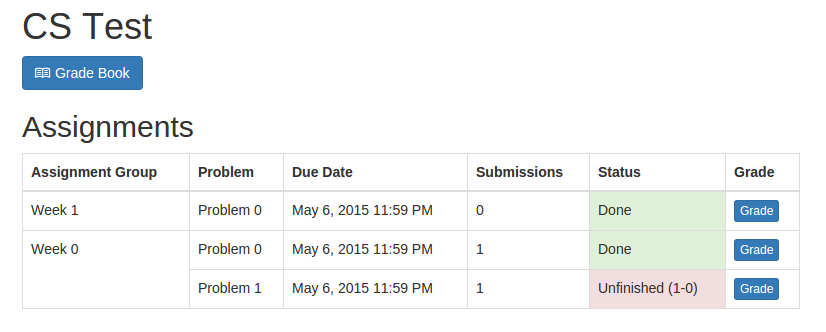
\includegraphics[width=\textwidth,height=\textheight,keepaspectratio]{diagrams/grutor_problems}
\caption{A list of all currently assigned problems in CS Test and the current grading status of the problems}
\label{fig:grutor_problems}
\end{figure}

On this page click the \emph{Grade} button for the problem you wish to grade. This will bring up a list of all
of the students in the class with the status of their submission, see Figure \ref{fig:grutor_problem_list}.

\begin{figure}[h]
\centering
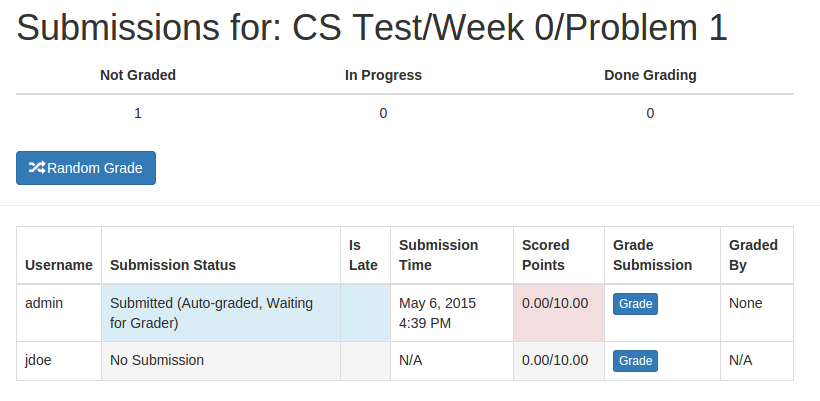
\includegraphics[width=\textwidth,height=\textheight,keepaspectratio]{diagrams/grutor_problem_list}
\caption{The current status of grading for all submissions in this problem}
\label{fig:grutor_problem_list}
\end{figure}

There are two ways to claim a submission to grade. First, you can click the \emph{Random Grade} button.
This button will atomically select a currently ungraded assignment for you. Second, you can click the
\emph{grade} button for the student you wish to grade. Once you have selected a problem to grade you will
see a page like in Figures \ref{fig:grade_page_top} and \ref{fig:grade_page_bottom}.

\begin{figure}
\centering
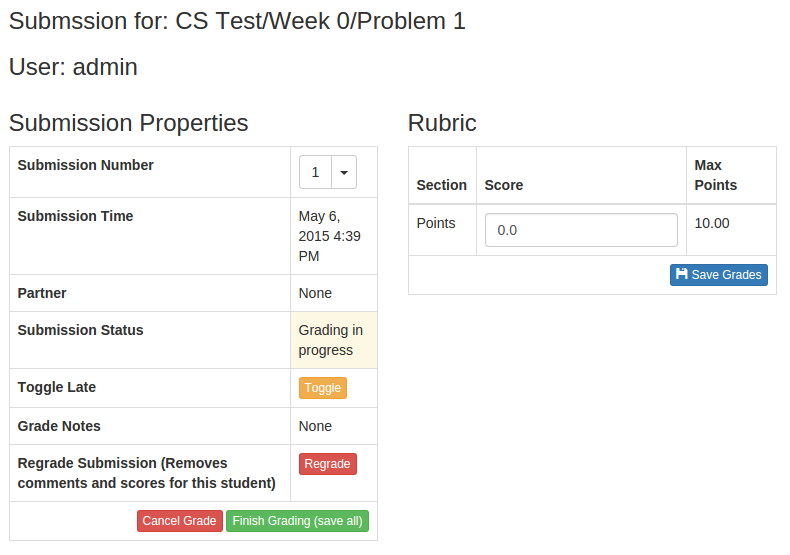
\includegraphics[width=\textwidth,height=\textheight,keepaspectratio]{diagrams/grade_top}
\caption{The top of the grading page}
\label{fig:grade_page_top}
\end{figure}

\begin{figure}
\centering
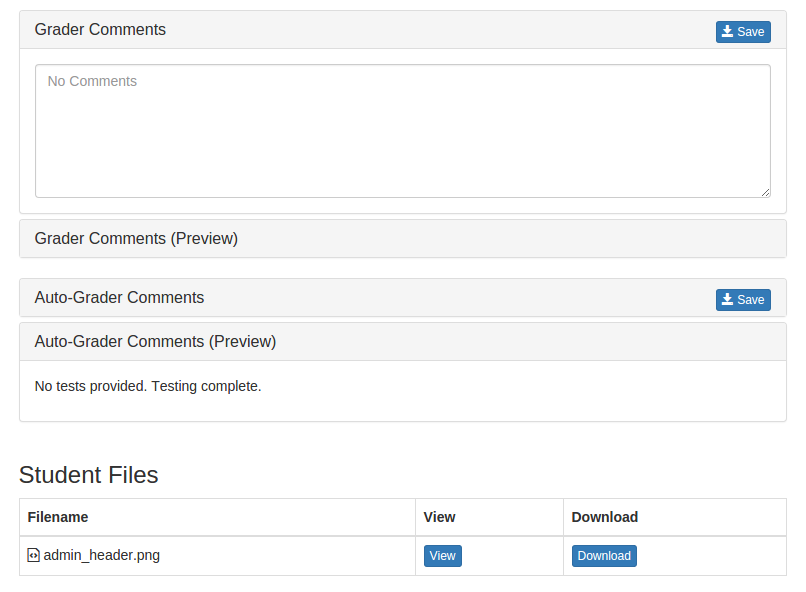
\includegraphics[width=\textwidth,height=\textheight,keepaspectratio]{diagrams/grade_bottom}
\caption{The comments and files section of the grading page}
\label{fig:grade_page_bottom}
\end{figure}

Grading is fairly simple, using the list of student files (Bottom of Figure \ref{fig:grade_page_bottom}) you
can view most textual, image, and PDF files. Files that cannot be directly viewed in browser may be
downloaded. 

To help during grading the professor can supply grading notes. These notes are in the \emph{Submission Properties}
table in the row labelled \emph{Grade Notes} (See Figure \ref{fig:grade_page_top}). If notes are supplied a button 
will be presented which will open the specified link in a new tab.

Once you have assessed the students submission and left comments (Figure \ref{fig:grade_page_bottom}) you must
save your changes and mark the submission as graded. All of this is handled by clicking the green
\emph{Finish Grading (save all)} button. Clicking this button will save all of the fields on the page and 
take you back to the list of submissions (Figure \ref{fig:grutor_problem_list}).

\noindent\textbf{Note:} If the submission you are working on has a partner that submission will receive the
exact same grades and comments that you put on this submission.

Additional things you can do on the grade page are modifying the late status of a submission, sending the
submission through the auto-grader again, and viewing old versions of the submission. These functions are 
all found in the \emph{Submission Properties} table (Figure \ref{fig:grade_page_top}).

\subsubsection{Status of Grading}

It is important to understand the different stages of grading for a submission. Each submission can be in
one of six stages:
\begin{enumerate}
\item Unsubmitted
\item Submitted: No auto-grading or grading
\item Auto-grading in progress
\item \label{item:autograded} Submitted: Auto-graded but not graded
\item \label{item:inprogress} Grading in progress
\item \label{item:graded} Graded
\end{enumerate}

Along with the status a submission also has a grader associated with it. For the most part submissions will always 
be in state \ref{item:autograded} when a grade gets to them. 
The largest area of confusion is how the \emph{Cancel Grade} and \emph{Finish Grading} buttons affect the
status of the submission. There are simple rules for how this works:
\begin{itemize}
\item You are listed as the grader of the submission.
\begin{description}
\item[Finish Grading] Sets the status to \ref{item:graded}. You are still the grader.
\item[Cancel Grading] Sets the status to \ref{item:autograded}. The submission has no grader.
\item[Leaving the page (other links)] Submission status does not change. Grader does not change.
\end{description}
\item Another grader is listed as the submission's grader
\begin{description}
\item[Finish Grading] Sets the status to \ref{item:graded}. You are now the grader.
\item[Cancel Grading] Submission status does not change. Grader does not change.
\item[Leaving the page (other links)] Submission status does not change. Grader does not change.
\end{description}
\end{itemize}

It is important to remember that if you leave the page via \emph{Cancel Grade} or any other link
none of your changes will be saved. If you want to make changes and leave with these methods you must
use the explicit blue save buttons for each section you modify.

\subsection{Entering grades in the Grade-book}
The other way graders can assign grades is through the grade-book. The grade-book is intended for assigning
grades to assignments or other parts of the class that were not submitted through the system, (e.g. 
Participation, Quizzes, Tests...).

To get to the Grade-Book click the Grader drop-down menu and select the course you wish to grade. This
brings up a page like in Figure \ref{fig:grutor_problems}. On this page click the \emph{Gradebook} button.
This will display a page like in Figure \ref{fig:gradebook}.

\begin{figure}
\centering
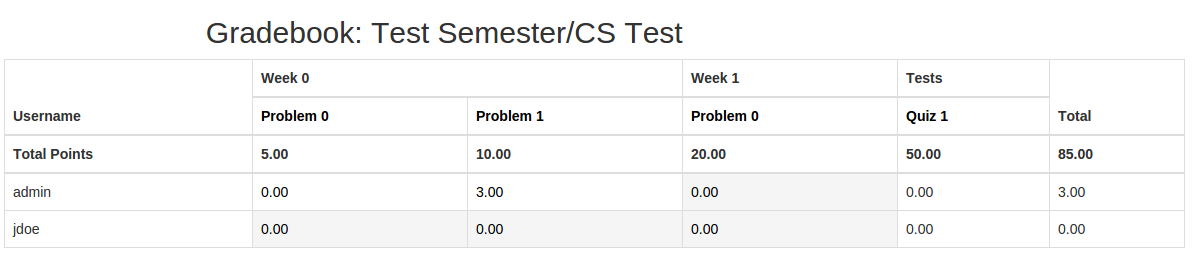
\includegraphics[width=\textwidth,height=\textheight,keepaspectratio]{diagrams/gradebook}
\caption{The grade-book for the course CS Test}
\label{fig:gradebook}
\end{figure}

Non-submitted grade-book columns are always the right most columns in the grade-book. For example in 
Figure \ref{fig:gradebook} The column \textbf{Quiz 1} in the category \textbf{Tests} is a non-submitted
column. 

To assign grades click the name of the column, in this case \textbf{Quiz 1}. This will take you to a page
like seen in Figure \ref{fig:gradecolumn}.

\begin{figure}
\centering
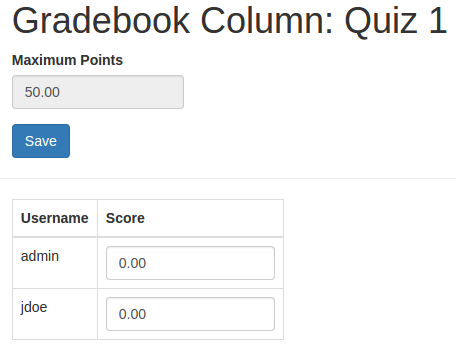
\includegraphics[width=\textwidth,height=\textheight,keepaspectratio]{diagrams/gradecolumn}
\caption{The grade column for Quiz 1 in CS Test}
\label{fig:gradecolumn}
\end{figure}

From here you may edit each students score. When you are done you can press save and leave. 
\textbf{Important Note:} Two graders cannot be editing the same grade-book column at the same time
once one grader saves their changes it will overwrite the other graders changes.

\pagebreak
\section{Instructor Use}
Instructors are responsible for configuring problems and adding columns to the grade-book as well as grading.
Since grading was covered in Section \ref{sec:graders} this section will focus on configuring courses and 
problems.

\subsection{General Course Settings}
Once an administrator has created a course and assigned you as an instructor you will need to begin configuring
your course. The course settings page is shown in Figure \ref{fig:course_settings}, this section will describe
the functionality of this page. \textbf{Note:} The figure does not show the entire page. At the bottom of the
page is the list of students, grutors, and instructors. This document will explain later how to use these lists.

First let us examine the \emph{Settings} panel near the bottom of the page. There are three major settings for
a course.

\begin{description}
\item[Course Homepage] This setting changes where the link in the \emph{Courses} drop down from the nav-bar
goes. By default it links to an empty built-in wiki page (use of the wiki is described in Section \ref{sec:wiki})
but it can be changed to link to an external site.
\item[Use Anonymous Grading] This boolean setting changes whether or not usernames are made anonymous to 
graders. If it is active any page under the \emph{Grader} drop-down for this course will use anonymous usernames. 
All pages in the \emph{Instructor} drop-down for this course will display both usernames.
\item[Late Work Policy] The late work policy changes how the system handles scoring assignments submitted late.
The default is \emph{Highlighter} which simply highlights late assignments red in the grade book. This policy can
be replaced via plug-in to modify scores based on how late or how many late assignments a student has turned in.
\end{description}

\noindent\textbf{Note (Possible feature request):} Currently the modified grade calculated by the late policy
is only displayed in the grade-book or the students \emph{My Grades} page. If a student views a problem 
individually it will show the original grade for that problem. This may be fixed in future versions of the
\csgt system.

\begin{figure}
\centering
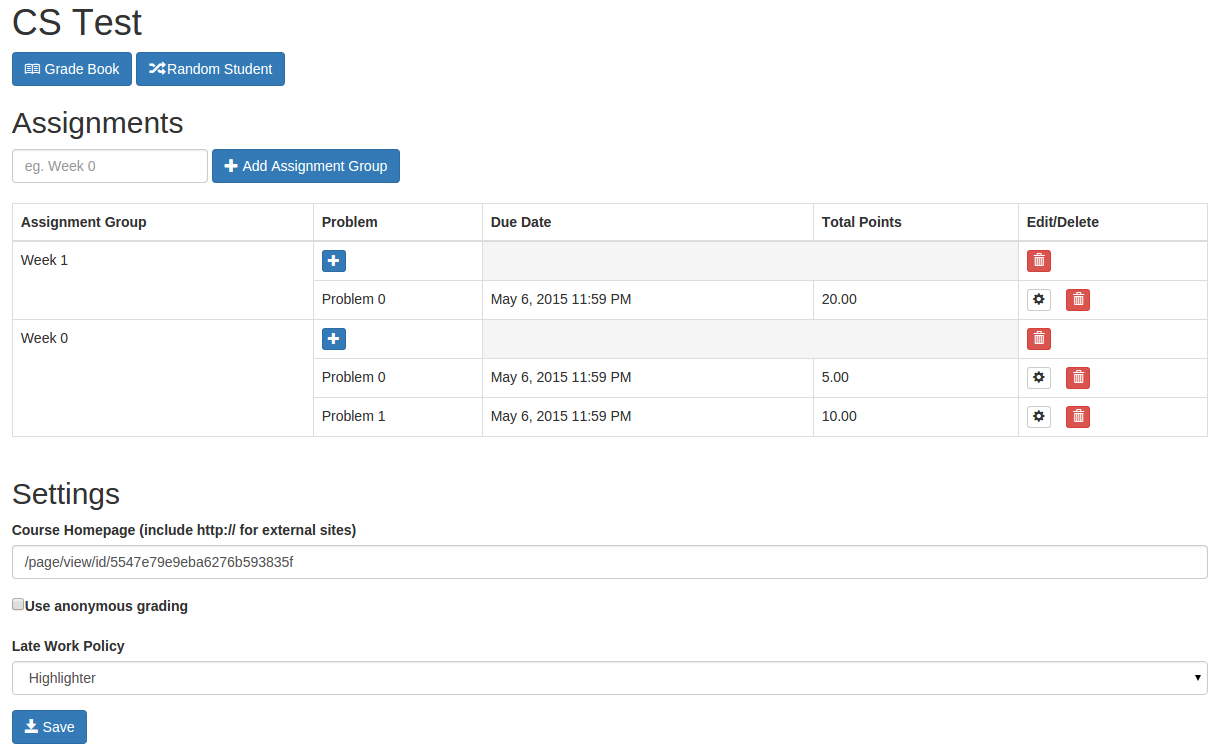
\includegraphics[width=\textwidth,height=\textheight,keepaspectratio]{diagrams/course_settings}
\caption{The main course settings page, minus the users lists}
\label{fig:course_settings}
\end{figure}

\subsection{Adding Problems}
Once you have configured the course to have the settings you want you will want to add problems.
Within the \csgt system problems are always contained within an \textbf{assignment group}. Assignment 
groups are ways to logically group related problems. For example assignment groups could be based on which week
the problems material relates to, which chapter of the book they relate to, or what problem set they are from.
Assignment groups are always displayed with the most recently assigned at the top of the page. This helps
students quickly locate the most relevant assignments.
	
To add a problem you must first create an assignment group. To create an assignment group type in the text-box
that displays the place-holder text \emph{eg. Week 0} and press the \emph{Add Assignment Group} button. In
Figure \ref{fig:course_settings} we can see that this course has assignment groups \textbf{Week 0} and 
\textbf{Week 1}. 

Once you have created an assignment group you can add a problem by clicking the blue plus button in the 
problem column for the assignment group you want. This will take you to the \textbf{Problem Settings} page, 
explained in Section \ref{sec:problem_settings}, you can also get to the problem settings page by clicking
the grey cog button for the problem you wish to modify.

\subsection{Problem Settings}
The problem settings page has four major sections: Problem Information, Problem Rubric, Problem Settings
(all seen in Figure \ref{fig:problem_settings}), and Tests. The first three sections are inter-related and
are all saved at once using the Save button at the bottom of the Problem Settings section. The tests are 
handled separately and will be described later in the chapter. 

\begin{figure}
\centering
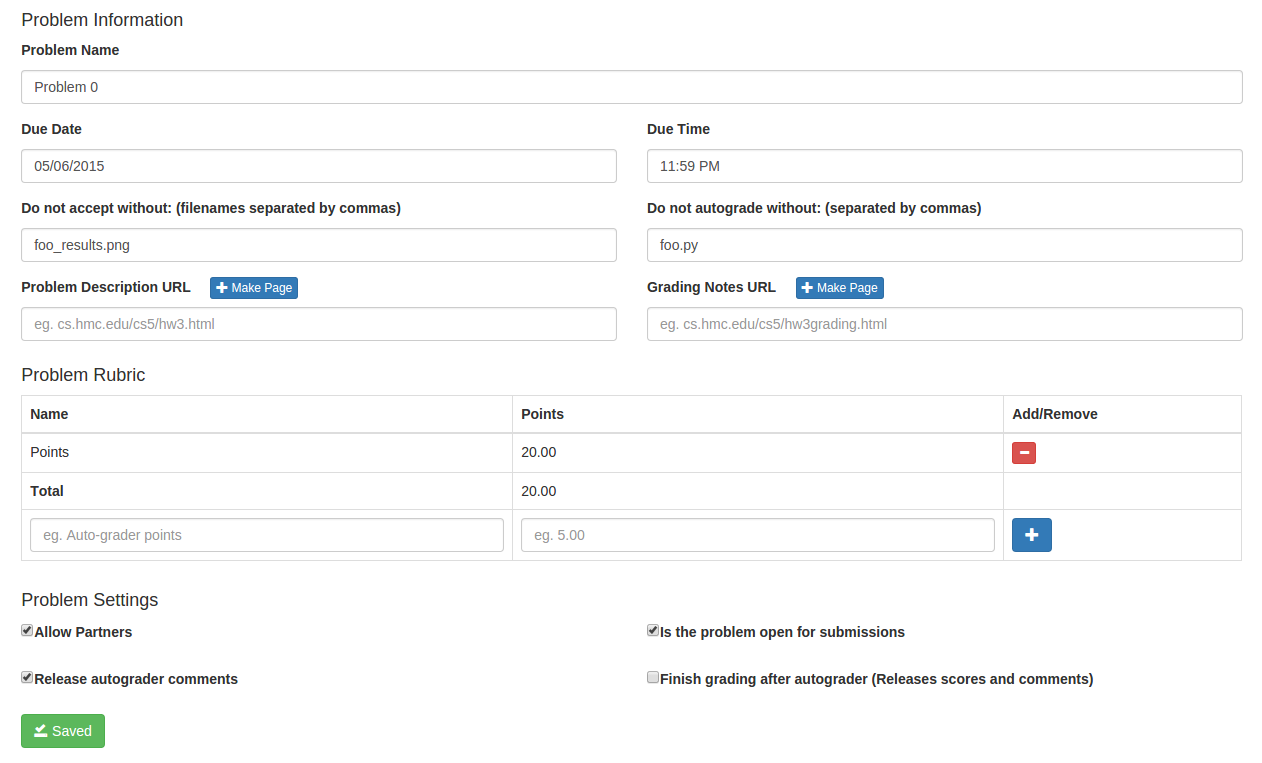
\includegraphics[width=\textwidth,height=\textheight,keepaspectratio]{diagrams/problem_settings}
\caption{The problem settings page}
\label{fig:problem_settings}
\end{figure}

\subsubsection{Problem Information}
The Problem Information section of the page allows you to enter basic information about the assignment.
Most of the sections are fairly self explanatory, but there are subtle distinctions about some:

\begin{description}
\item[Do not accept without] A comma separated list of files which the system should reject a submission
if any of them are missing. This is useful to prevent students from turning in partial assignments.
\item[Do not auto-grade without] A comma separated list of files which the system should look for to
be allowed to run the auto-grader. This is good if you want to accept partial submissions but some files
may be required to not crash the auto-grading system.
\item[Problem Description URL] A link to the specification of the problem. This can be an external link
(preceded with \texttt{http://}) or a wiki page (See section \ref{sec:wiki}). The \emph{Make Page} button
will generate a wiki page where you can write the specification for the problem.
\item[Grading Notes URL] A link to the specification for graders to use to grade problems. This link is only
made available to graders. Similarly to the Problem Description URL it can be a wiki page generated with the
\emph{Make Page} button.
\end{description}

\subsubsection{Problem Rubric}
The problem rubric is where you can specify how many points a problem is worth. Rubrics may contain
multiple sections to help both graders and students better understand what deductions are for. 

Sections can be added to the rubric by typing a name and a number of points into the fields at the bottom
of the table then clicking the \emph{plus} button. Similarly you can remove a section by clicking the 
\emph{minus} button. Modifications are color coded and only applied when the save button is pressed

\noindent\textbf{Note:} To change the number of points assigned by a section simply re-add that section.

\noindent\textbf{Note:} Removing a section of the rubric does not remove any points assigned to a student 
in that particular field of the rubric. If you need to remove a section of the rubric that has already been
graded you will need to use the command line to remove or rename the assigned points. Example in section
\ref{sec:assigning_points:fixing_rubrics}.

\subsubsection{Problem Settings}
The settings section contains four toggles to change the way the problem handles submissions.

\begin{description}
\item[Allow Partners] If this box is checked the student submission page allows students to select one partner
to submit with. Otherwise that box is disabled.
\item[Is this problem open for submissions] When this box is checked the students can click the submit button.
when it is unchecked that button is removed.
\item[Release Autograder Comments] When this box is checked any comments that the auto-grader makes are shown
to the students before their grade is marked as done. Otherwise a student looking at their grade will see a 
place-holder comment telling them to check back when the grading is finished.
\item[Finish grading after autograder] When this is checked the auto-grader will mark a submission as done
grading once it has finished. If the auto-grader fails to grade an assignment it will be left in the 
\emph{Waiting for Autograder} state. 
\end{description}

\subsection{Tests}
One of the major features of the system is its ability to auto-grade student submissions. To allow this each
problem has a section in its settings page to add multiple test files (See figure \ref{fig:problem_tests}).

\begin{figure}
\centering
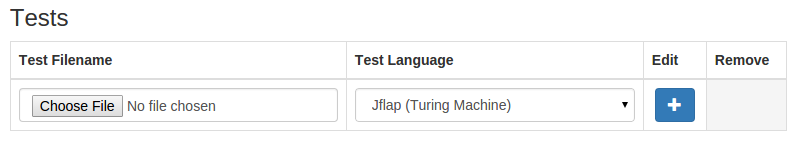
\includegraphics[width=\textwidth,height=\textheight,keepaspectratio]{diagrams/problem_tests}
\caption{The problem tests lists}
\label{fig:problem_tests}
\end{figure}

\subsubsection{Adding Tests}
Adding a test is fairly simple. First select the unit-test file you want to upload.
Next select the type of unit test that the file is for. The currently implemented test types are:

\begin{description}
\item[Python (pyunit)] This type runs a pyunit test file.
\item[Java (junit4)] This type runs a Junit4 style test file.
\item[Prolog (plunit)] This type runs a Prolog file that implements plunit tests.
\item[Racket (rackunit)] This type runs a rackunit test file. \textbf{Note:} There are 
several subtleties to running the rackunit tests which are described in Section \ref{sec:writing_tests}.
\item[Picobot] This type runs a picobot program in various mazes from various starting positions. 
An online picobot simulator can be found at the HMC Picobot site
\url{http://www.cs.hmc.edu/picobot/}.
\item[JFLAP] This type runs various inputs through DFAs and NFAs defined using the JFLAP program. 
\textbf{Note:} The JFLAP simulator that this type uses is based off of a python script that was developed
over many years for use internal to HMC. It may contain some bugs in edge cases that don't occur in standard
HMC assignments.
\item[JFLAP (Turing Machine)] This type runs various inputs through turnig machines defined using the JFLAP program. 
\textbf{Note:} The JFLAP simulator that this type uses is based off of a python script that was developed
over many years for use internal to HMC. It may contain some bugs in edge cases that don't occur in standard
HMC assignments.
\item[Supplemental File] Supplemental files are never executed. Instead these files are meant to allow
the test files to get external data or link in extra code pieces. 
\end{description}

\subsection{Test Settings}
By default when you add a test file to a problem it will parse the file to look for tests. Each test it 
finds it will assign one point to an unspecified rubric section. This functionality provides a useful
default but it is often useful to have more power when specifying which tests go to what rubric sections
and how many points they are worth. 

To allow for this functionality the site provides a test settings page, 
seen in Figure \ref{fig:test_settings}.
\begin{figure}
\centering
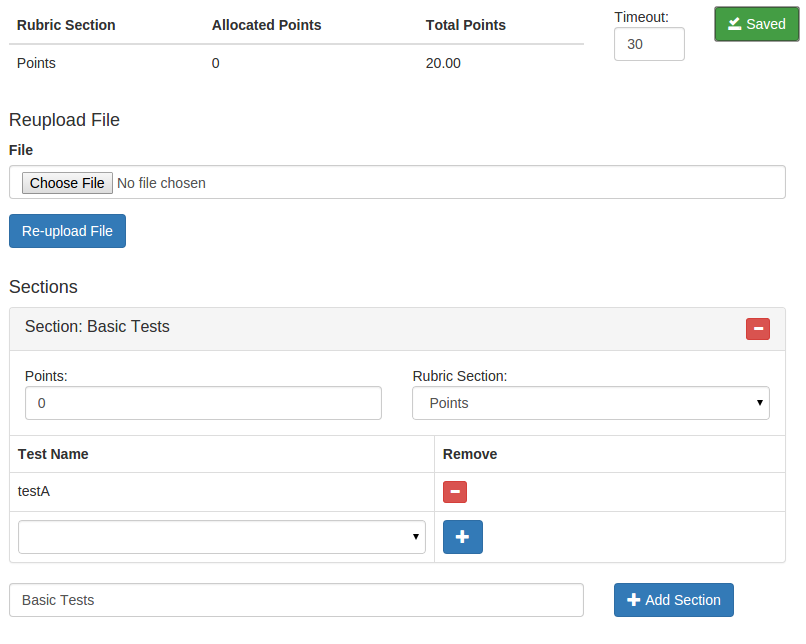
\includegraphics[width=\textwidth,height=\textheight,keepaspectratio]{diagrams/test_settings}
\caption{The test point allocation page}
\label{fig:test_settings}
\end{figure}

To allocate points you must first create a \emph{Test Section}. Once you have a test section you can 
define how many points it is worth, which rubric section it assigns points to, and which tests are 
part of that section. 

\noindent\textbf{Note:} Any test that is not in a section will not be displayed to the student. If you want
a test to be run but not have any points assigned to it you should put it in its own 0 point section.


\subsection{Writing Tests}
\label{sec:writing_tests}
There are some idiosyncrasies with some of the auto-grader systems (mostly stemming from the fact 
that some languages do not easily support external unit-tests). This section covers some of the 
test writing issues that attempt to combat those idiosyncrasies.

\subsubsection{Generic Test Features}
One of the biggest features of the testing framework is being able to provide external output.
To help the system differentiate between student code output, test framework output, and output 
intended to be presented to the student, the system uses a simple annotation system. 

When a test wants to produce output that is presented to the student in the web interface the print
statement should begin with the name of the test and a colon. This is probably best shown in an example:

\begin{verbatim}
def testThatPrints(self):
  x = studentCode()
  print "testThatPrints: Your code produced %d" % (x) 
\end{verbatim}

This will print out \texttt{Your code produced \#} to the student in the grading comments
(where \# is whatever number their code produced). 

\pagebreak
\subsubsection{Python}
Python has relatively few issues but there are some things to point out. First it is recommended to us 
\texttt{import foo as bar}. This helps prevent name conflicts with the unit-testing framework or your 
test classes. Below is a simple example file:

\begin{verbatim}
import hw3pr2 as hw
import unittest


class BasicTests(unittest.TestCase):
  def testA(self):
    self.assertEqual(hw.foo(3), 2)
    


if __name__ == '__main__':
  unittest.main()
\end{verbatim}

Another important point is that a python test file must be executable on its own. 
This means that it must contain a "main". 

\pagebreak
\subsubsection{Java}
Java, like python, has relatively few issues with the auto-grader. Currently the only tested style of
test writing is using the \texttt{@Test} decorator. Below is a simple test file:

\begin{verbatim}
import static org.junit.Assert.*;
import org.junit.Test;

public class BasicTests {

  /* This tests whether the foo function multiplies by 3 */
  @Test
  public void testA() {
    assertTrue( foo(2) == 6 );
  }
}
\end{verbatim}

The biggest issue with the Java auto-grader is the way its test detection regex works. Even though
Java will let you put a comment between the decorator and the function the regex doesn't do a very
good job detecting the test name without the decorator being directly adjacent to the function 
definition.

\pagebreak
\subsubsection{Racket}
Racket is one of the more complicated testing systems. Because students submit self contained racket 
files racket doesn't want to import the student's code into the test file. To combat this the auto-grader 
performs temporary modifications to the students code, such as removing the \texttt{\#lang racket}
declaration. 

Additionally if a student has failed to implement a function to in their submitted code the grading will
fail. To combat this it is recommended to create a different test file for each function you wish to
test. Because each test file is executed independently a failure in one file will not affect the others.

The Racket auto-grader uses the \emph{rackunit} framework. This framework allows us to add comments to
the tests which we use as test names. Because of limitations of the test name extraction regular expression
tests must be at most split across 2 lines. This makes for terribly unattractive test files and we are working
on improving its capabilities. An example test file is below:

\begin{verbatim}
;;;Racket - Unit Tests Example

#lang racket
(include "change.rkt")
(require rackunit)

(check-equal? (min-change 1 '(1 5 10 25 50)) '(1)
	"one-cent")
(check-equal? (min-change 42 '(1 5 10 25 50)) '(1 1 5 10 25)
	"42-cents us coins: your test didn't make 42 cents change with us coins")
(check-equal? (min-change 42 '(1 5 21 35)) '(21 21)
	"42-cents weird coins")
(check-equal? (min-change 0 '(1 5 21 35)) '()
	"no change")
\end{verbatim}

In this case the names of the tests are anything in in the comment strings before a colon. If there is no
colon the name is the whole string. 

\pagebreak
\subsubsection{Prolog}
Prolog has relatively few issues with the auto-grader. The test system utilizes the basic Prolog
unit-testing framework. When importing the student's submitted code it is important to turn off 
loading unit-tests. An example file is below:

\begin{verbatim}
:- set_test_options([load(never)]).
:- include('sort.pl').
:- set_test_options([load(always)]).

:- begin_tests(selectionSort).
test(selectionSortT1) :- selectionSort([1, 2, 3], [1, 2, 3]), !.
:- end_tests(selectionSort).
\end{verbatim}

\subsubsection{JFLAP and JFLAP (Turing Machine)}
The JFLAP and JFLAP (Turing Machine) use a simple text file format to specify tests. 
The format consists simply of an input string to be fed to the automaton and then 
if that input should reject. The biggest issue is that the auto-grader only knows what
file to run the tests on based on the name of the solution file. For example the file 
\texttt{part1.sols} will grade the JFLAP file \texttt{part1.jff}. An example file follows

\begin{verbatim}
 reject
100101
100100 reject
1
00 reject
\end{verbatim}

Inputs that reject are followed by a space and the word reject. All others accept. To indicate the empty 
string as an input simply leave a blank line or a just the space and the word reject.

\subsubsection{Picobot}
Similar to JFLAP, Picobot uses a text input file. The format consists of which map to test the 
program on, what file the program is contained in and then a list of starting positions. An example
file is below

\begin{verbatim}
emptyMap
hw0pr3.txt
###
topleftcorner: 1,1
toprightcorner: 23,1
bottomrightcorner: 23,23
middle: 10, 10
othermiddle: 9,9
\end{verbatim}

There are three available maps:
\begin{enumerate}
\item \texttt{emptyMap} Figure \ref{fig:empty_map}
\item \texttt{mazeMap} Figure \ref{fig:maze_map}
\item \texttt{extraMap} Figure \ref{fig:extra_map}
\end{enumerate}

\begin{figure}
	\centering
	\begin{subfigure}[b]{0.3\textwidth}
		
\includegraphics[width=\textwidth]{diagrams/emptyMap}
		\caption{The empty map}
		\label{fig:empty_map}
	\end{subfigure}
	\begin{subfigure}[b]{0.3\textwidth}
		
\includegraphics[width=\textwidth]{diagrams/mazeMap}
		\caption{The maze map}
		\label{fig:maze_map}
	\end{subfigure}
	\begin{subfigure}[b]{0.3\textwidth}
		
\includegraphics[width=\textwidth]{diagrams/extraMap}
		\caption{The extra map}
		\label{fig:extra_map}
	\end{subfigure}
	\caption{The various maps available to the Picobot auto-grader}
	\label{fig:maps}
\end{figure}

\pagebreak
\section{Wiki Use}
\label{sec:wiki}
The \csgt system provides a wiki like system for providing problem descriptions, grading notes, and
even full course websites. 

\noindent\textbf{Note:} The wiki system saw relatively little use during our first semester of testing. 
Because of this the wiki system may contain more issues than other parts of the \csgt system.

\subsection{Wiki page permissions}
One of the most critical points of the wiki system is the ability to set the view and edit permissions.
The permissions table is seen in Figure \ref{fig:wiki_permissions}.

\begin{figure}
\centering
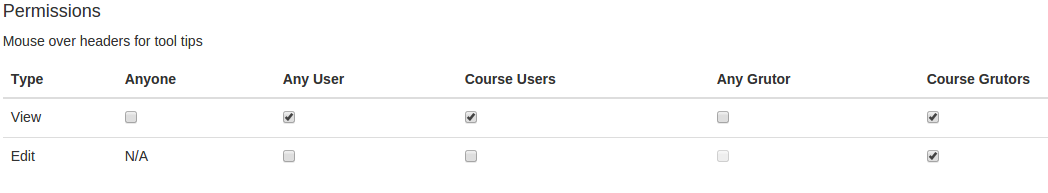
\includegraphics[width=\textwidth,height=\textheight,keepaspectratio]{diagrams/wiki_permissions}
\caption{The wiki page permissions table}
\label{fig:wiki_permissions}
\end{figure}

For each category of users you can assign either \emph{view} or \emph{edit} permissions. The only 
restrictions are that if a group does not have view permission they cannot have edit permissions and
you cannot give edit permissions to users who are not registered for the site. The vertical columns
have the following meanings:

\begin{description}
\item[Anyone] Any person on the internet. The page does not check for credentials.
\item[Any User] Any person who has a login with this instance of the \csgt system. 
\item[Course Users] Any person who is registered as a student in the course that owns this page.
\item[Any Grutor] Any person who is registered as a user for any course.
\item[Course Grutors] Any person who is registered as a grutor for the course that owns this page.
\end{description}

Course instructors always have access and the ability to edit a page. 

\subsection{Wiki syntax}
The basic wiki syntax is based on Markdown (\url{http://daringfireball.net/projects/markdown/syntax})
but there are several extensions to allow for designing nicer looking pages. 

The first major extension enabled is the Attribute list extension 
(\url{http://pythonhosted.org//Markdown/extensions/attr_list.html}).
This extension allows you to specify attributes such as CSS classes and styles. Additionally
you can specify IDs to use as anchors for links. 

The second major extension is a custom wiki link syntax extension. Default links in markdown allow
you to link to external sites. Because links are long strings of UUID's for the wiki it is impractical
to use them to create links (\textbf{Note:} It is planned to add easier links in the future). To solve 
this the markdown syntax has been expanded to include a wiki link as follows:

\begin{verbatim}
[Text]<Semester Name, Course Name, Page Title>
[Text]<Course Name, Page Title>
[Text]<Page Title>
\end{verbatim} 

The difference in the three lines is that the less information you provide the more it will grab from
the course that owns the current page.

Like in most wikis if a page you reference doesn't exist that page will be created. That page will inherit
the permissions of the page that created it. 

Along with links and text you can upload an image and load that into a page. To access an image you use
something like the link syntax but starting with a "!".

\begin{verbatim}
![Alt Text]<Semester Name, Course Name, Page Title, Image Name>
![Alt Text]<Course Name, Page Title, Image Name>
![Alt Text]<Page Title, Image Name>
![Alt Text]<Image Name>
\end{verbatim}

Like links it will load information not provided from the page that the link exists in. You can also use
the attribute list to specify a width and height of the image.

\pagebreak
Below is a small example page:
\begin{verbatim}
Welcome to the homepage of the CS Test course for Test Semester!

# HI IM A RED HEADER # {style="color:red;"}
This is stuff that is blue
{style="color:blue;"}

<pre>
Test code blocks
</pre>

[Text]<Test Semester, CS Test, Test Page> 

[Other]<Fake Semester, CS Test, Test Page>

[Not created yet]<Test Semester, CS Test, Not Created>

![Alt Test]<Alien.PNG>
\end{verbatim}

The rendered page is shown in Figure \ref{fig:wiki_example}.

\begin{figure}
\centering
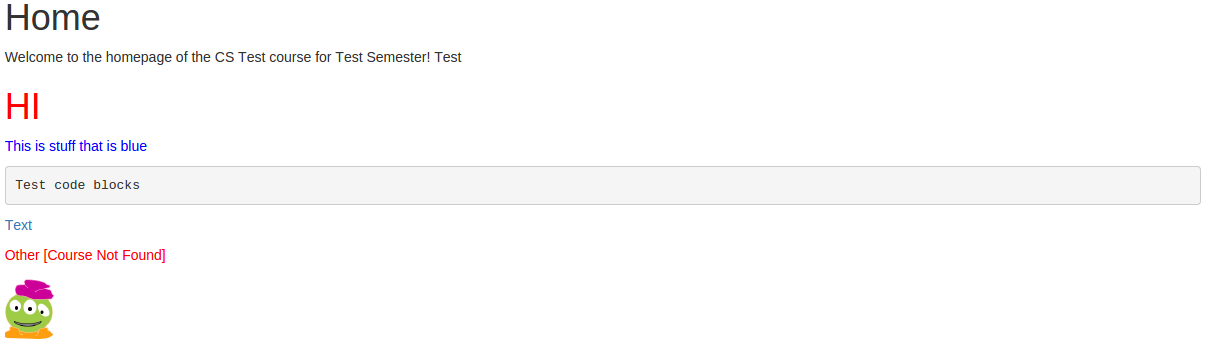
\includegraphics[width=\textwidth,height=\textheight,keepaspectratio]{diagrams/example_wiki}
\caption{An example wiki page}
\label{fig:wiki_example}
\end{figure}



\chapter{Administration}
\label{ch:admin}
\section{Server Structure}
The \csgt system is designed to be modular and expandable as the number of users of the system grows.
To accommodate this each of the five major components are designed to be operated as a separate server.
The five components are:

\begin{enumerate}
\item Python-Flask Front-end Server
\item Python-Celery Grading Worker
\item File-system for submission storage (pick your favorite one)
\item MongoDB for storing grades
\item RabbitMQ for passing grading requests to workers
\end{enumerate}

In the most basic configuration, which is most useful for testing, all of the required components will be
on one machine. As the requirement for redundancy and scalability increases components may be moved to
separate servers and replicated. Figure \ref{fig:layout} shows one possible configuration of the servers
which provides redundancy on both the front and back end. It is important to note that a load-balancer is
required to support multiple front-ends.

\textbf{Note:} Currently even though MongoDB and rabbitMQ support distributed options the system has never
been tested using that configuration. This is a feature which may be researched in the future if it becomes
needed.

\begin{figure}
\centering
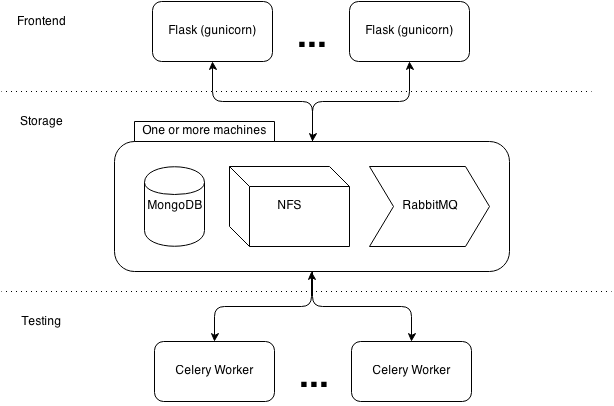
\includegraphics[width=\textwidth,height=\textheight,keepaspectratio]{diagrams/HMC_Grader_Layout}
\caption{Possible server configuration for \csgt}
\label{fig:layout}
\end{figure}





\section{Set-up}
Once you have decided on the basic configuration for your servers setting up the requisite systems requires a
little work. For each server type I will provide basic set-up instructions. These instructions are listed in
order to prevent dependency issues.

\subsection{MongoDB Set-up}
To set-up a brand new MongoDB instance you can use the instructions below. If you already have a running version
of MongoDB you can adapt the instructions or request help from your database administrator.
\begin{enumerate}
\item Get the latest version of MongoDB from \href{http://docs.mongodb.org/manual/tutorial/install-mongodb-on-ubuntu/}{here}.
\item Follow \href{http://docs.mongodb.org/manual/tutorial/enable-authentication/}{these} instructions to create an administrator account.
\item Edit \verb|/etc/mongodb.conf| so that
\verb|bind_ip| is commented and uncomment
\verb|auth = true|. Additionally it is recommended to change the port that the server listens on
to prevent attacks.
\item Reload \emph{mongod} and log into the \emph{mongo} shell with\\
\verb|$ mongo -u {username} -p --authenticationDatabase admin|
\item Type \verb|> use submissionsite| to create the \emph{submissionsite} database
\item Add a user for this database by typing
\begin{verbatim}
> db.createUser(
  { user: "grader",
    pwd: "{your password}",
    roles: [{role: "dbOwner", db: "submissionsite"}]
  }
)
\end{verbatim}
\item Finally \verb|> quit()| the mongo shell.
\end{enumerate}

\subsection{File-system Set-up}
Setting up the file-system is pretty easy. There are two major requirements for the file-system, one, it
must be accessible from all machines in the cluster, and two it must have a minimal required directory
structure.

Because exporting a directory is complicated and other better resources exist on the internet I leave
figuring out how to export your directory as an exercise to the reader.

Once you decide how to export your chosen storage directory you must give it some basic structure. This
structure is as follows:

\begin{itemize}
	\item submissions
	\item photos
	\item plugins
	\begin{itemize}
		\item autograder
		\item latework
	\end{itemize}
\end{itemize}

Once these paths exist in your storage directory you are good to go.

\subsection{RabbitMQ Set-up}

RabbitMQ is a distributed queue which handles sending auto-grading requests to the various celery workers.
Setting up this part of the system can be very easy but depending on your security requirements you may want
to enforce more stringent permissions. To set-up RabbitMQ do the following:

\begin{enumerate}
\item Install \emph{rabbitmq-server}.
\item Run\\ \verb|$ sudo rabbitmqctl add_user {username} {password}|
\item Run\\ \verb|$ sudo rabbitmqctl set_permissions -p / {username} ".*" ".*" ".*"|
\end{enumerate}

RabbitMQ is now in a very basic workable configuration.

\subsection{Create config.py}
\label{sec:config}
The \texttt{config.py} file handles all of the connection configuration for the system.
Inside \texttt{config.py} there are several sections that need to be modified using configuration
information from the steps above.

\begin{enumerate}
\item Give your own \verb|SECRET_KEY|
\item Configure MongoDB connection properties
\begin{verbatim}
MONGODB_SETTINGS = {
'DB': 'submissionsite',
'username': '{dbuser}',
'password': '{dbpassword}',
'host': '{db_ip}'
'port': '{db_port}'
}
\end{verbatim}
\item Configure the Celery broker URL\\
\verb|CELERY_BROKER_URL="amqp://{rabbit_user}:{rabbit_pwd}@{rabbit_ip}"|
\item Set the where the file-system will be mounted for the front/back-end servers\\
\verb|STORAGE_HOME="{path_to_mount_point}"|\\
\textbf{Note:} If you are storing the data locally you still have to set this flag but instead
want to set \verb|STORAGE_MOUNTED=False|. This disables a check to make sure that the directory is
mounted before performing writes.
\item Set up the system email (This is used for sending password reset requests
\begin{verbatim}
SYSTEM_EMAIL_ADDRESS = "{server_email}"
SMTP_SERVER = "{smtp_server}"
\end{verbatim}
\end{enumerate}

This configuration file should be passed to all front/back-end servers.
\\
\\
\noindent\textbf{Note:} There is an additional setting \verb|GRADER_USER| which is currently set to
\verb|None|. This setting is supposed to set which user to switch to as the auto-grader but it
is currently non-functional.

\subsection{Flask Front-end Set-up}
The Flask based Front-end of the system serves dynamically generated web-pages to the users.
To set-up the flask front-end do the following:

\begin{enumerate}
\item Ensure that \verb|python-dev| (or its equivalent package) is installed on your platform.
\item Check out the repository
\item \verb|$ cd <your_repository>|
\item Copy \texttt{config.py} to the repository
\item Create a virtual environment using \verb|virtualenv <venv_name>|
\item \textbf{Temporary Fix} The current version of mongoengine does not function with the latest version
of pymongo. To solve this install version 2.8 \verb|$ <venv_name>/bin/pip install pymongo==2.8|
\item Install the following packages with pip\\
\texttt{\$ <venv\_name>/bin/pip install flask flask-script flask-bootstrap flask-login flask-markdown mongoengine flask-mongoengine WTForms python-dateutil celery psutil python-magic bleach gunicorn gevent flower}
\item Launch the front-end processes\\
\verb|$ <venv_name>/bin/celery flower -A app:celery|\\
\verb|$ <venv_name>/bin/gunicorn -w 4 -k gevent -b 0.0.0.0:80 app:app|
\end{enumerate}

\noindent\textbf{Note:} You may have to modify some permissions to allow \emph{gunicorn} to bind to port 80.
Additionally if you are using a load balancer you may want to bind it to some other higher port.

\subsection{Celery Worker Back-end Set-up}
Setup for the Celery Worker is almost identical to the Flask front-end but requires fewer packages. The
instructions are displayed below:

\begin{enumerate}
\item Ensure that \verb|python-dev| (or its equivalent package) is installed on your platform.
\item Check out the repository
\item \verb|$ cd <your_repository>|
\item Copy \texttt{config.py} to the repository
\item Create a virtual environment using \verb|virtualenv <venv_name>|
\item \textbf{Temporary Fix} The current version of mongoengine does not function with the latest version
of pymongo. To solve this install version 2.8 \verb|$ <venv_name>/bin/pip install pymongo==2.8|
\item Install the following packages with pip\\
\texttt{\$ <venv\_name>/bin/pip install flask flask-script flask-bootstrap flask-login flask-markdown mongoengine flask-mongoengine WTForms python-dateutil celery psutil python-magic bleach}
\item Launch the worker processes\\
\verb|$ <venv_name>/bin/celery worker -A app:celery|
\end{enumerate}

\subsection{Bootstrap the Administrator Account}
All of the previous sections have gotten a working version of the system but currently there are no accounts
in the database. To begin creating accounts there must be an administrator account.

The easiest way to create the \texttt{admin} account is to run\\
\verb|$ <venv_name>/bin/python run.py|\\
then kill this process. \texttt{run.py} launches the debug server which also checks for an administrator account
if no account is found it creates it. You can find the password for the default \texttt{admin} account in
\texttt{run.py}.





\section{Managing Courses}
\subsection{Creating Courses}
The administrator is required to create all of the courses for the system. When a course is created all administrators are invisibly added as instructors. Any other instructors must be explicitly added by an
administrator.

To add a new course to the system first navigate to the \emph{Admin Dashboard} (See Figure \ref{fig:admindash}).
Once in the Admin Dashboard click the link for the \emph{Courses} panel. Fill in the required information and
click the \emph{Create Course} button.

\begin{figure}
\centering
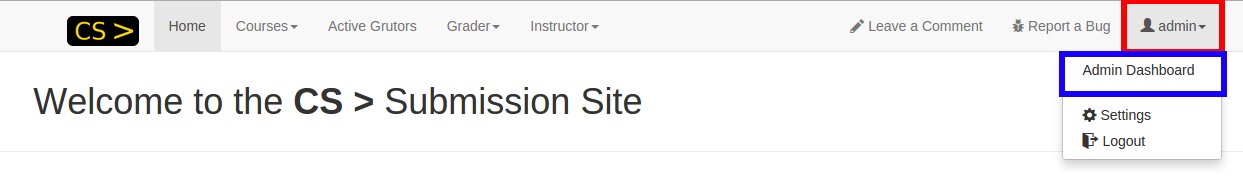
\includegraphics[width=\textwidth,height=\textheight,keepaspectratio]{diagrams/admin_header}
\caption{Red: The user Dropdown, Blue: The admin dashboard link}
\label{fig:admindash}
\end{figure}

\subsection{Adding Instructors}
Once a course has been created instructors (other than the current administrators) must be added to the course.
This requires the following actions:
\begin{enumerate}
\item Navigate to the course settings page. If you just created the course find it in the \emph{Active Courses}
list and click \emph{Administer}. If you are on the main page click the \emph{Instructor} drop-down and click on
the course link.
\item Scroll to the bottom of the course settings page.
\item Under the instructors heading enter the user-name of the desired instructor. (If the instructor does not have an account yet see Section \ref{sec:createusers}). Click the plus button.
\item That user is now an instructor.
\end{enumerate}

\subsection{Deactivating Courses}
When a course is finished it is desired to prevent that course from being modified. Additionally we want
currently activated courses to be prioritized when displaying lists of courses to users.
To accomplish this \csgt allows the administrator to \textbf{Deactivate} a course. When a course is deactivated
it no longer accepts submissions and is moved from the main drop down menus into a separate page of old courses.

To deactivate a course first navigate to the Admin Dashboard and then to the Courses panel. Once on the courses
panel find the desired course and click the \emph{Deactivate} button.
\\
\\
\noindent\textbf{Note:} Some of the archival pages are still works in progress, but the framework is there to
accomplish these features. If you run into problems with deactivated courses please submit a bug report.



\section{Creating User Accounts}
\label{sec:createusers}
One of the primary roles of the \texttt{admin} account is to create user accounts. There are two methods
for creating accounts for users.

\subsection{Creating via web}
Web creation is the easiest way to create a small number of accounts. The steps are as follows:

\begin{enumerate}
\item Navigate to the \emph{Admin Dashboard} by clicking the user drop-down menu and then \emph{Admin Dashboard}. Figure \ref{fig:admindash} shows the locations of the links.

\item Once in the \emph{Admin Dashboard} navigate to the user panel using the top bar. (See Figure \ref{fig:adminuser})
\item Fill in the information fields and click \textbf{Create User}. (See Figure \ref{fig:adminuser})

\begin{figure}[h]
\centering
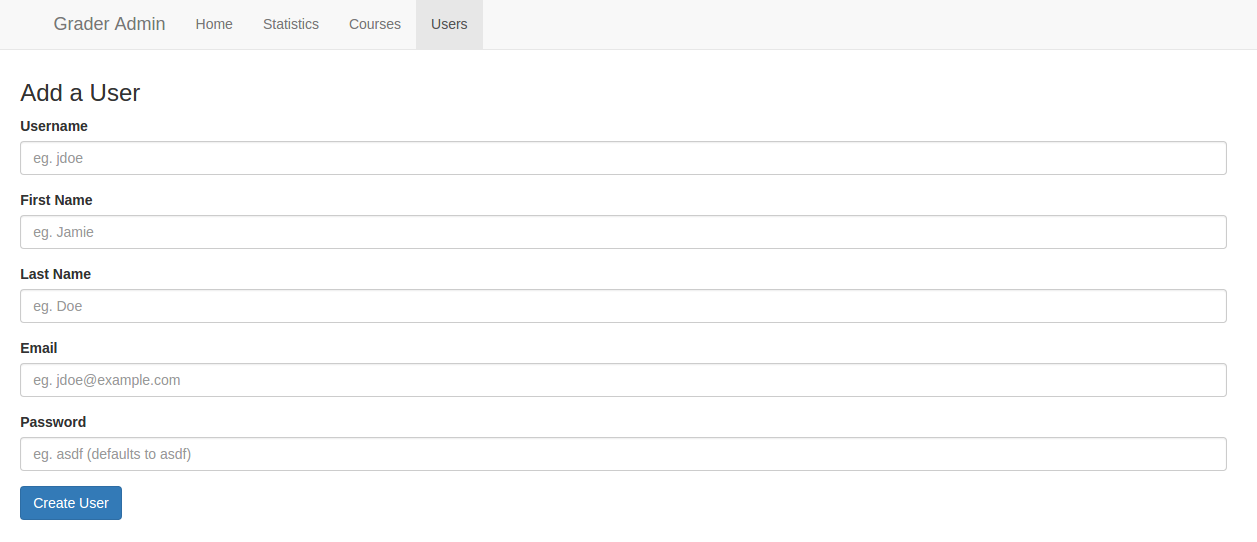
\includegraphics[width=\textwidth,height=\textheight,keepaspectratio]{diagrams/admin_users}
\caption{The admin users panel}
\label{fig:adminuser}
\end{figure}
\end{enumerate}

\subsection{Creating via command line}
Creating new users via the command line is generally one of the easiest ways to add large batches of users.
There are already several scripts (Located in \verb|app/scripts| in the repository) which demonstrate how to
add users from various files (CSV files with different column layouts). Below are general instructions for adding
a user via command line:
\\
\\
\noindent\textbf{Note:} To correctly use the mongo interface for the system in python you must export \verb|PYTHONPATH| as the root directory of the repository.

\begin{verbatim}
$ export PYTHONPATH=<path_to_repository>
$ <venv_name>/bin/python
...python start message...
>>> from app.structures.models.user import *
>>> user = User()
>>> user.username = "<username>"
>>> user.firstName = "<firstName>"
>>> user.lastName = "<lastName>"
>>> user.email = "<email>"
>>> user.setPassword("<password>")
>>> user.save()
\end{verbatim}

\noindent If we then want to add the user to a course we want to continue by doing

\begin{verbatim}
>>> from app.structures.models.course import *
>>> c = Course.objects.get(semester="<semester>", name="<name>")
>>> #One or more of these
>>> user.courseStudent.append(c)
>>> user.courseGrutor.append(c)
>>> user.courseInstructor.append(c)
>>> user.save()
\end{verbatim}




\chapter{Development}
\label{ch:develop}
Foo

\chapter{Command Line Reference}
Some functionality is too infrequently used or too cumbersome to provide through
the web interface. Including:

\begin{itemize}
  \item Assigning all students a comment and a score for a given prolem.
  \item Changing the password of a student.
  \item Adding a user to a large number of courses at once.
  \item Making a user an administrator.
  \item Creating a large number of user acounts from a file.
\end{itemize}

Other functionality simply hasn't been made available yet
in the web interface and will be added later. Including:
\begin{itemize}
  \item Marking all submission grading status as "Done".
  \item Sending all submissions through the auto-grader again.
\end{itemize}

This section will demonstrate how to use the scripts provided to perform these
functions as well as other useful tips for the command line.

\section{Setting up the Environment}
Because of the way the python import system works, before you can run any
scripts or do work on the command line you must first export the environment
variable \texttt{PYTHONPATH} to the location of the root of your repository.
One easy way to do this is:
\begin{verbatim}
$ cd <your_repository>
$ export PYTHONPATH=`pwd`
\end{verbatim}

\section{Using the provided scripts}
The repository contains several useful scripts in the directory
\texttt{app/scripts}.

\subsection{Adding batches of users}
The three scripts \texttt{addUsersFromList}, \texttt{addUsersFromSakai},
\texttt{addGrutorsFromList} all provide examples for how to read \texttt{CSV}
style files and creating user accounts from them.

Theses scripts were designed for the data format used by the Harvey Mudd
College Registrar and so may not be immediately useful at other schools, but
they will provide good reference.

\subsection{Assigning Points}
\label{sec:assigning_points}

\subsubsection{Removing points from removed rubric sections}
\label{sec:assigning_points:fixing_rubrics}
When a section is removed from the rubric the system doesn't remove any assigned points from submissions.
To handle this situation you must delete or move the assigned points in the submission's grade object.
\begin{verbatim}
>>> s = #A submission object obtained by magic (Python)
>>> #Move points from a badly named section
>>> s.grade.scores['Points'] = s.grade.scores['Pionts']
>>> #Remove an unneeded section
>>> del s.grade.scores['useless']
>>> s.save() #Don't forget to save
\end{verbatim}
\end{document}
